\documentclass[10pt,showpacs,preprintnumbers,footinbib,amsmath,amssymb,aps,prl,twocolumn,groupedaddress,superscriptaddress,showkeys]{revtex4-1}
\usepackage{graphicx}
\usepackage{subcaption}
\usepackage{dcolumn}
\usepackage{bm}
\usepackage[colorlinks=true,urlcolor=blue,citecolor=blue]{hyperref}
\usepackage{color}
\usepackage{amsmath}
\usepackage{multirow}
\usepackage{natbib}

\newcommand{\costa}[1]{% \costa{<power>}
	\ensuremath{\cos ^{#1} {\theta}} }
\newcommand{\sinta}[1]{% \sinta{<power>}
	\ensuremath{\sin ^{#1} {\theta}} }
\newcommand{\pwrten}[1]{%\pwrten{<power>}
	\ensuremath{10^{#1}} }
\newcommand{\rhomax}{
	\ensuremath{ \rho _{\mathrm{max}}} }
\newcommand{\fourpisqr}{
	\ensuremath{ 4 \pi ^2} }
\newcommand{\deriv}[3][]{% \deriv[<order>]{<function>}{<variable>}
	\ensuremath{ \frac{d ^{#1} {#2}}{d {#3}^{#1}}}}

\begin{document}
\title{PHY 905 Project 4: Molecular Dynamics}
\author{Thomas Redpath}
\affiliation{Department of Physics, Michigan State University}
\begin{abstract}

\end{abstract}
\maketitle

\section{Introduction}

Molecular dynamics


\section{Theory}

\subsection*{Lennard-Jones Potential}


\begin{equation}
	U(r_{ij}) = 4\epsilon\left[\left(\frac{\sigma}{r_{ij}}\right)^{12} - \left(\frac{\sigma}{r_{ij}}\right)^6\right],
	\label{eq:lj}
\end{equation}

\begin{figure}
	\centering
	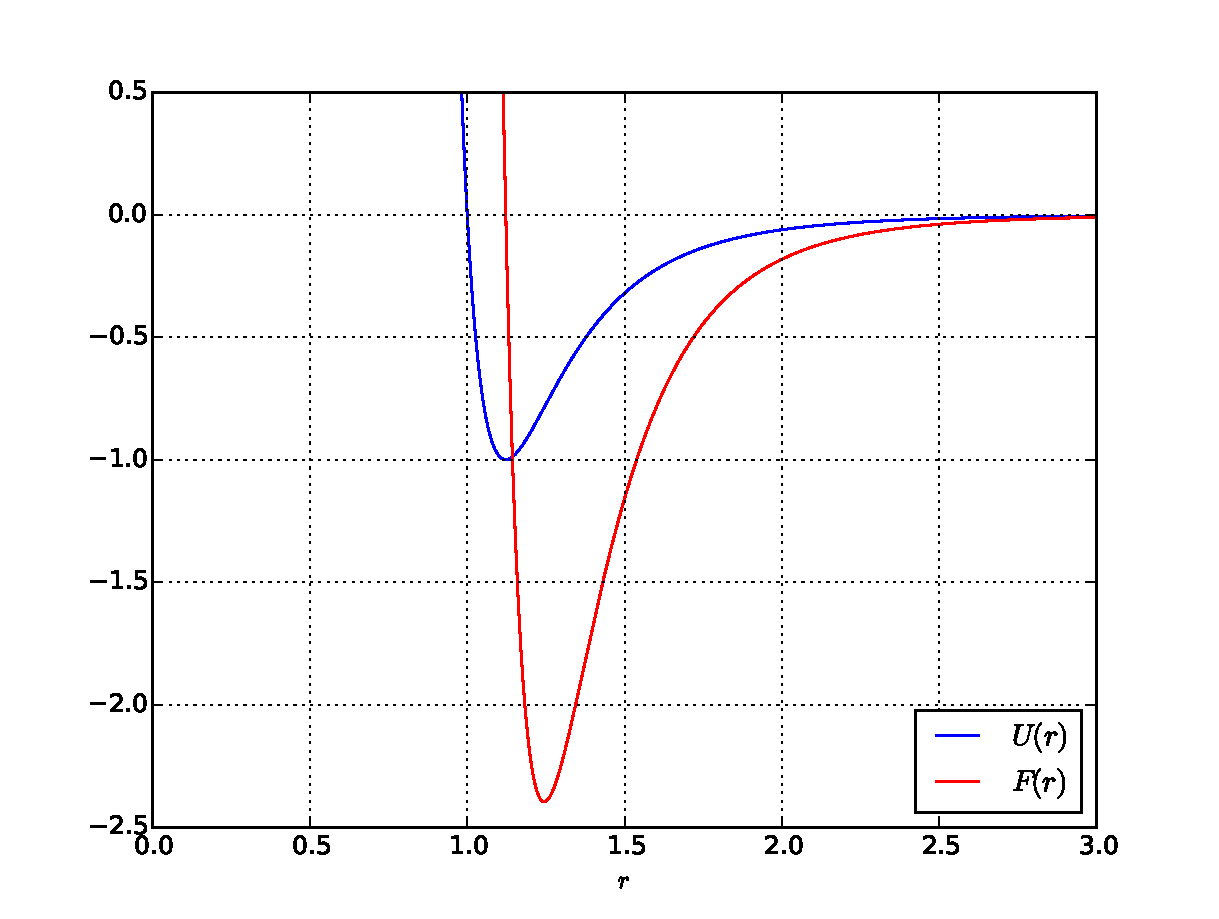
\includegraphics[width=0.5\textwidth]{figures/LJ.pdf}
	\caption{The Lennard-Jones potential (blue) and derived force (red).}
	\label{fig:lj}
\end{figure}

\subsection*{Units}

The small scale of the system we are simulating lends itself to working in a
specialized set of units. We used the following four relations to define our
system of units

\begin{align*}
	\text{1 unit of mass } &= 1 \text{ a.m.u} = 1.661\times 10^{-27}\mathrm{kg},\\
	\text{1 unit of length } &= 1.0 {\AA} = 1.0\times 10^{-10}\mathrm{m},\\
	\text{1 unit of energy } &= 1.651\times 10^{-21}\mathrm{J},\\
	\text{1 unit of temperature} &= 119.735\mathrm{K}.
\end{align*}
Converting to this system of units, Boltzmann's constant becomes
$k = (1.38 \times \pwrten{-23} )(119.7)(1.65 \times \pwrten{-21}) = 1$.

\subsection*{Thermodynamic quantities}

Temperature
\begin{equation}
	T = \frac{2}{3}\frac{E_k}{N_\text{atoms} k_B}.
	\label{eq:temperature}
\end{equation}

Diffusion constant
\begin{equation}
	D = \frac{\langle r^2(t) \rangle }{6t}
	\label{eq:diffusion}
\end{equation}


\section*{Algorithms and Methods}

The C++ code developed for this project utilizes the velocity
Verlet method to solve Newton's equations of motion. In this section we briefly
summarize the derivation of this method discussed in \citet{Morten}. We
then provide a description of the codes which can be
found at \url{https://github.com/redpath11/phy905_thr} in the
\texttt{projects/project4/src} directory.

\subsection*{Verlet Method}

We numerically solve the equations of motion using the velocity
Verlet method. Since we've assumed a Lennard-Jones type
pairwise interaction between atoms, the form of the acceleration
is known from the gradient of the interaction potential. The Verlet
method derives from a summation of two Taylor expansions. Consider
the position in one dimension

\begin{align*}
	x(t+h) &= x(t) + h x'(t) + \frac{1}{2} h^2  x''(t) + O(h^3)\\
	x(t-h) &= x(t)  - h x'(t) + \frac{1}{2} h^2  x''(t) + O(h^3).
\end{align*}
Summing these two expansions and switching to the discretized
notation gives

\begin{equation*}
	x_{i+1} = 2 x_i - x_{i-1} + h^2 x''_i + O(h^4).
\end{equation*}
In general, this algorithm is not self-starting since it requires the
value of $x$ at two previous points.

Now, consider a Taylor expansion of the velocity and note the
relationshipe between velocity and acceleration $v' = a$.

\begin{align*}
	v_{i+t} &= v_i + h v_i ' + \frac{1}{2} v_i '' + O(h^3)\\
	a_{i+1} &= v'_i + h v''_i + O(h^2).
\end{align*}
We will assume that the velocity is a linear function of time
$hv''_i \approx v'_{i+1} - v'_i$. We can now write the final
algorithmic form for the position and velocities.

\begin{align}
%%\begin{split}
	x_{i+1} &= x_i + hv_i + \frac{h^2}{2} v'_i + O(h^3)\\
	v_{i+1} &= v_i + \frac{h}{2}(v'_{i+1} + v'_i) + O(h^3)
\label{eq:Verlet}
%%\end{split}
\end{align}

\subsection*{Code}

\subsubsection*{Overview}

We were supplied a code skeleton (from
\url{ https://github.com/andeplane/molecular-dynamics-fys3150})
 outlining the major classes needed to run a molecular dynamics
simulation. From this starting point, we filled in details to apply
periodic boundary conditions, initialize the system of argon
atoms in face-centered cubic (FCC) lattice, calculate the pairwise
forces from the Lennard-Jones potential and compute physical
properites of the system. Figure~\ref{fig:flowchart} gives a
general overview of the code structure by identifying key
elements and where they reside in the within the class structure.

\begin{figure*}
	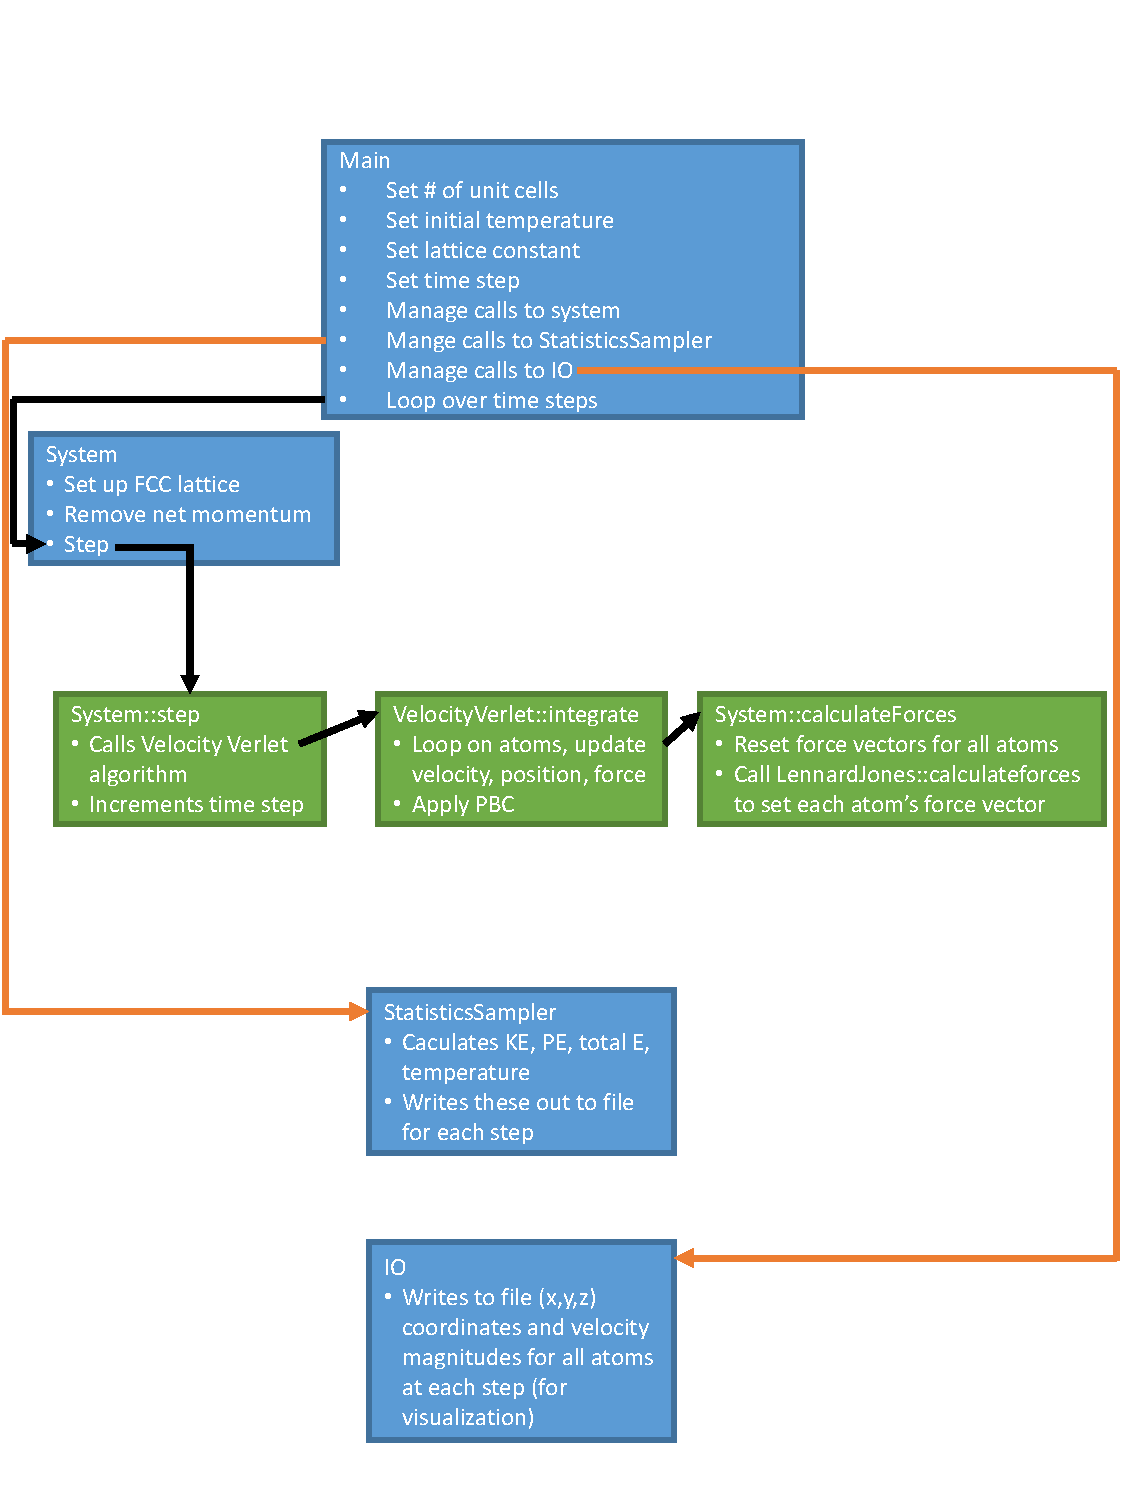
\includegraphics[width=\textwidth]{figures/flowchart.pdf}
	\caption{The flowchart gives a crude overview of how the
	code operates. Blue boxes represent classes and
	indicate processes carried out by one or more memeber
	functions. Green boxes represent functions crucial to the 
	simulation. Black arrows indicate the hierarchy of function
	calls for one timestep. Orange arrows depict function
	calls that result in writing data to a file.}
	\label{fig:flowchart}
\end{figure*}
	

\subsubsection*{Initialization}

Initialization of our system takes place in two general steps: (1)
setting the size, initial temperature and Lennard-Jones potential
characteristics and (2) setting the initial positions and velocities
for the atoms. The first step is implemented in the \texttt{main}
function. The size of the system is determined by the number of
unit cells in the FCC lattice and the lattice constant (the size of
one unit cell). We studied a system of argon atoms for which
the lattice constant is 5.26 {\AA} \textbf{REFERENCE}. The
$\epsilon,\sigma$ parameters specify the L-J potential, for argon
these are $\epsilon / k_B = 119.8\mathrm{K}$, $ \sigma=3.405
{\AA}$.

The second initialization step is carried out in the \texttt{System}
class. This class contains a function \texttt{System::createFCCLattice}
to position $4 \times N_x \times N_y \times N_z$ atoms in a cubic lattice
and give them random velocities drawn from a Maxwell-Boltzmann
distribution.
% (eq.~\ref{eq:MBdist}).

\begin{equation*}
	P(v_i) = \sqrt{\frac{m}{2 \pi k T}} \exp \left [ \frac{-m v_i ^2}{2kT} \right ]
%	\label{eq:MBdist}
\end{equation*}
Doing so gives the system some
initial kinetic energy (i.e. temperature). It should be noted that this
does not generate a system
in equilibrium, but rather it populates some random microstate with a
random initial kinetic energy. The \texttt{System::removeTotalVelocity}
function subtracts the net velocity from each atom so that the center of
mass of the system is stationary.

An initialized system consisting of 500 atoms (5 unit cells) is shown in FIG.
~\ref{fig:init300K}. We used Ovito \citep{ovito} to visualize the system.

Density?

\begin{figure}
\centering
	\begin{subfigure}[b]{0.5\textwidth}
	\centering
		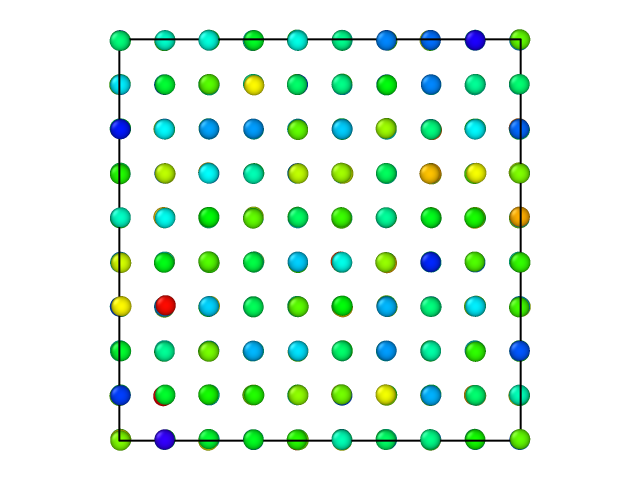
\includegraphics[width=\textwidth]{figures/Init300Kxy.png}
		\caption{Top view}
		\label{fig:init300kxy}
	\end{subfigure}
\\
	\begin{subfigure}[b]{0.5\textwidth}
	\centering
		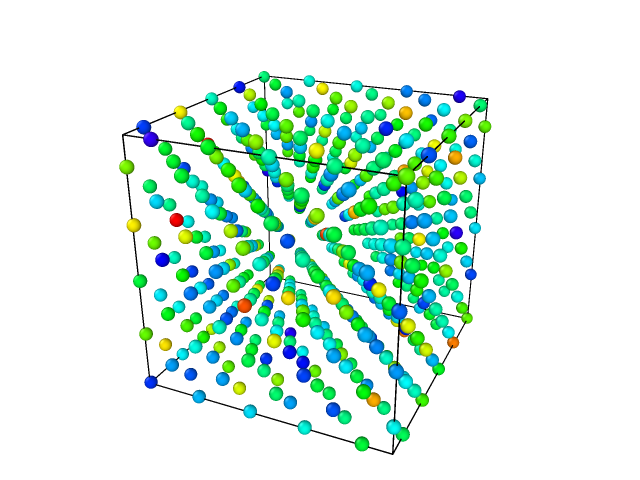
\includegraphics[width=\textwidth]{figures/Init300K3d.png}
		\caption{3d view}
		\label{fig:init300k3d}
	\end{subfigure}
	\caption{Positions and velocity magnitudes (indicated by the color)
	visualized in Ovito for the system initial state.}
	\label{fig:init300K}
\end{figure}

\subsubsection*{Simulation}

general flow

how observables are sampled; mention that $D$ is calculated for every
step

efficiency



Melting point?



\subsubsection*{Output}



\section*{Results and discussion}

\subsection*{Energy Conservation}

Our first test of the simulation was to ensure that energy conservation
is obeyed. This test revealed a major bug in the way we were applying
the periodic boundary conditions. When this is not done correctly, the
potential energy and forces are incorrectly calculated because the
distances between atoms is wrong. Once this issue was resolved, we
obtained the results shown in Table~\ref{tab:dt14eV} for a simulation
of 1000 time steps and an initial temperature of 300 K.

% Table generated by Excel2LaTeX from sheet 'Sheet1'
\begin{table*}[htbp]
  \centering
  \caption{Results from a simulation with the initial temperature $T_0=300$ K and a
  time step size $dt = \pwrten{-14}$ s. Values in the time column are in MD units
  ($1.00224 \times \pwrten{-13}$ s). }
    \begin{tabular}{rrrrrr}
    \toprule
    Timestep & Time  & Temperature [K] & KineticEnergy [eV] & PotentialEnergy [eV] & TotalEnergy [eV] \\
%    \midrule
\hline
    1     & 0.099777 & 312.026 & 20.1662 & -38.3532 & -18.187 \\
    101   & 10.0774 & 158.627 & 10.252 & -28.4274 & -18.1754 \\
    201   & 20.0551 & 163.31 & 10.5547 & -28.7268 & -18.1721 \\
    301   & 30.0327 & 171.405 & 11.0779 & -29.252 & -18.1741 \\
    401   & 40.0104 & 160.382 & 10.3655 & -28.5349 & -18.1694 \\
    501   & 49.988 & 169.434 & 10.9505 & -29.1232 & -18.1726 \\
    601   & 59.9657 & 159.62 & 10.3162 & -28.4912 & -18.175 \\
    701   & 69.9434 & 164.443 & 10.6279 & -28.8028 & -18.1748 \\
    801   & 79.921 & 167.812 & 10.8457 & -29.0173 & -18.1716 \\
    901   & 89.8987 & 172.008 & 11.1168 & -29.2901 & -18.1732 \\
%    \bottomrule
\hline
    \end{tabular}%
  \label{tab:dt14eV}%
\end{table*}%


\subsection*{Equillibrium Temperature}

In a preceeding section about initializing the simulation, we mentioned
that the ``initial'' temperature we set is not the actual temperature of the
system but rather a way to set the total energy of the system.
When we randomly assign velocities to each atom,
we are starting the system in a random one of its virtually uncountable
microstates. Through simulating the interactions between atoms, we
evolve the system through other microstates at each time step where,
according to the ergodic hypothesis, the probability of reaching a
given microstate is given by the probability distribution governing
the ensemble. Now, the initial state that we populate when we construct
the system isn't likely to be an equilibrium state for the system, but as we
run the simulation, the system evolves to reach a region of the phase
space corresponding to equilibrium microstates. This process is represented
by the peak at 0 and subsequent fall off in FIG.~\ref{fig:tempsteps}.
Once the system reaches equilibrium (around step 175), the temperature
fluctuates randomly around its equilibrium value ($T_{eq}$). We found
that the equilibrium temperature is roughly half the initial temperature.

\begin{figure}
\centering
	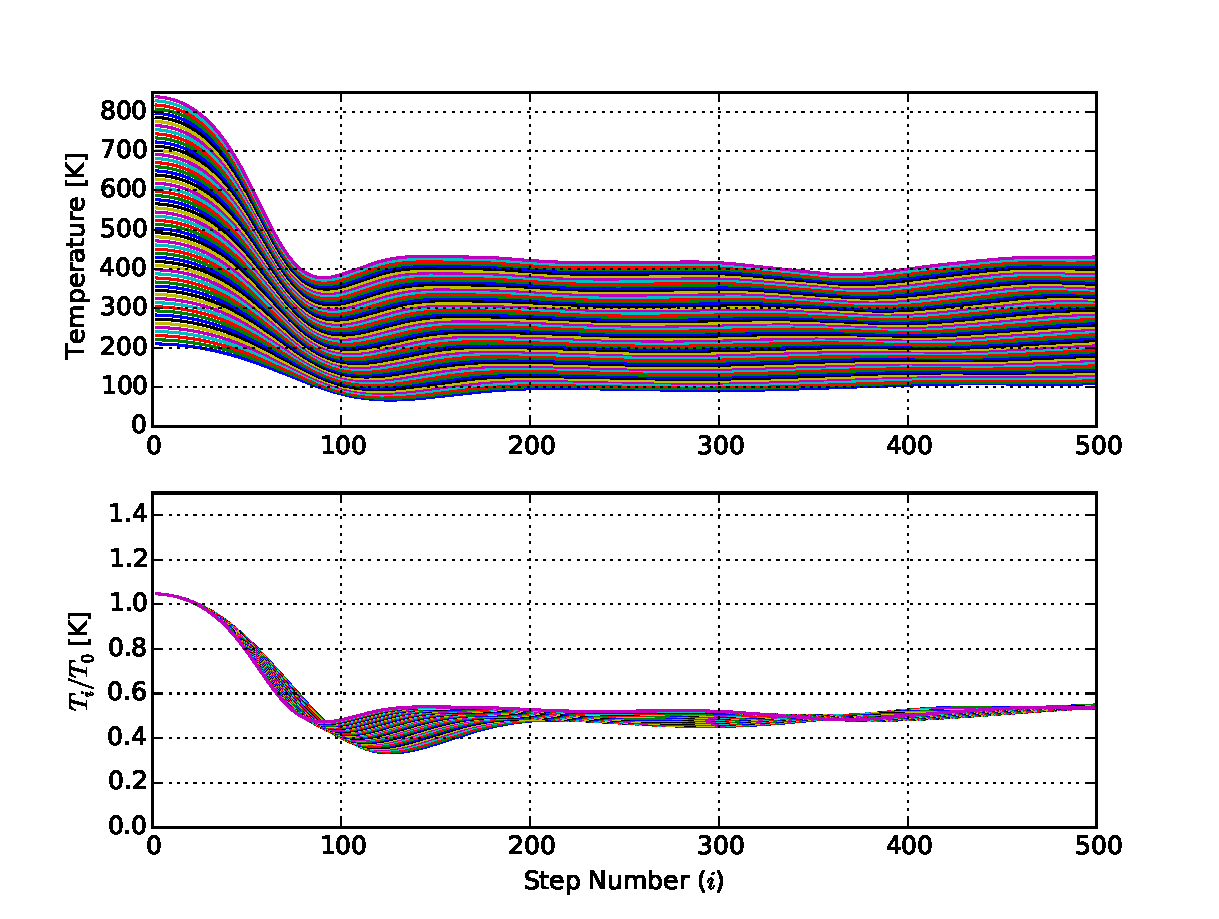
\includegraphics[width=0.5\textwidth]{figures/TempSteps.pdf}
	\caption{The top panel plots calculated system temperature
	(eq.\ref{eq:temperature}) vs. time step
	number for starting temperatures $T_0$ ranging from 200 to 800
	K (the different lines). The bottom panel presents the same data
	as the top panel but with the temperature at each step normalized
	by the $T_0$ for that simulation. We varied the initial temperature
	between 200 K and 800 K and used a time step
	value $dt = \pwrten{-15}$ s.
	For all the simulations, the
	equillibrium temperature is roughly half the initial temperature.}
	\label{fig:tempsteps}
\end{figure}

%states that the time spent by
%a system in some region of the phase space containing microstates with
%the same energy is proportionaly to the volume of this region.

\subsection*{Diffusion Constant}

Next, we investigated the melting point of the system by comparing the
diffusion constant from simulations with different starting temperatures
$T_0$ (or equivalently $T_{eq} \approx T_0/2$).
In FIG.~\ref{fig:TDplot}, we show the sampled temperature and
diffusion constant vs. step number from simulations with $T_i$ ranging
from 100 K to 900 K. These simulations used a step size $dt = \pwrten{-14}$
s and ran for 1000 steps. We looked at the diffusion coefficent as a
function of time to gain insight into the state of the system. Recall that
a system of atoms in a solid state will be constrained to the vicinity of
their lattice sites and therefore the system will have a smaller average
displacement when compared to a system in a liquid state. In this case,
the atoms move more freely so the system will exhibit a larger average
displacement. Since the diffusion constant ($D$) is proportional to the
average
displacement (eq.~\ref{eq:diffusion}), it provides an indication of the
state of the system.

In the bottom panel of FIG.~\ref{fig:TDplot},
we see that $D$, towards the end of the simulation, separates the
simulations into two groups.
The lower band, indicates $T_0$ values for which $D$ remains constant
over the course of the simulation. In the upper group, $D$ gradually rises
over the course of the simulation. For the largest $T_0$ simulations,
$D$ reaches a steady state before the end of the simulation. We
interpret this increase in $D$ as a phase transition where the system
changes from a solid to a liquid (it melts). Furthermore, the slope
indicates how quickly the process happens - for systems initialized
with a large amount of kinetic energy (higher $T_0$), the transition
occurs faster than for systems initialized with a lower $T_0$. Closer
inspection of FIG.~\ref{fig:TDplot} reveals a small group of systems
with a higher final $D$ than the non melting cases. These systems
are likely very close to the melting point so the phase transition
takes a long time or they only partially melt.

\begin{figure}
\centering
	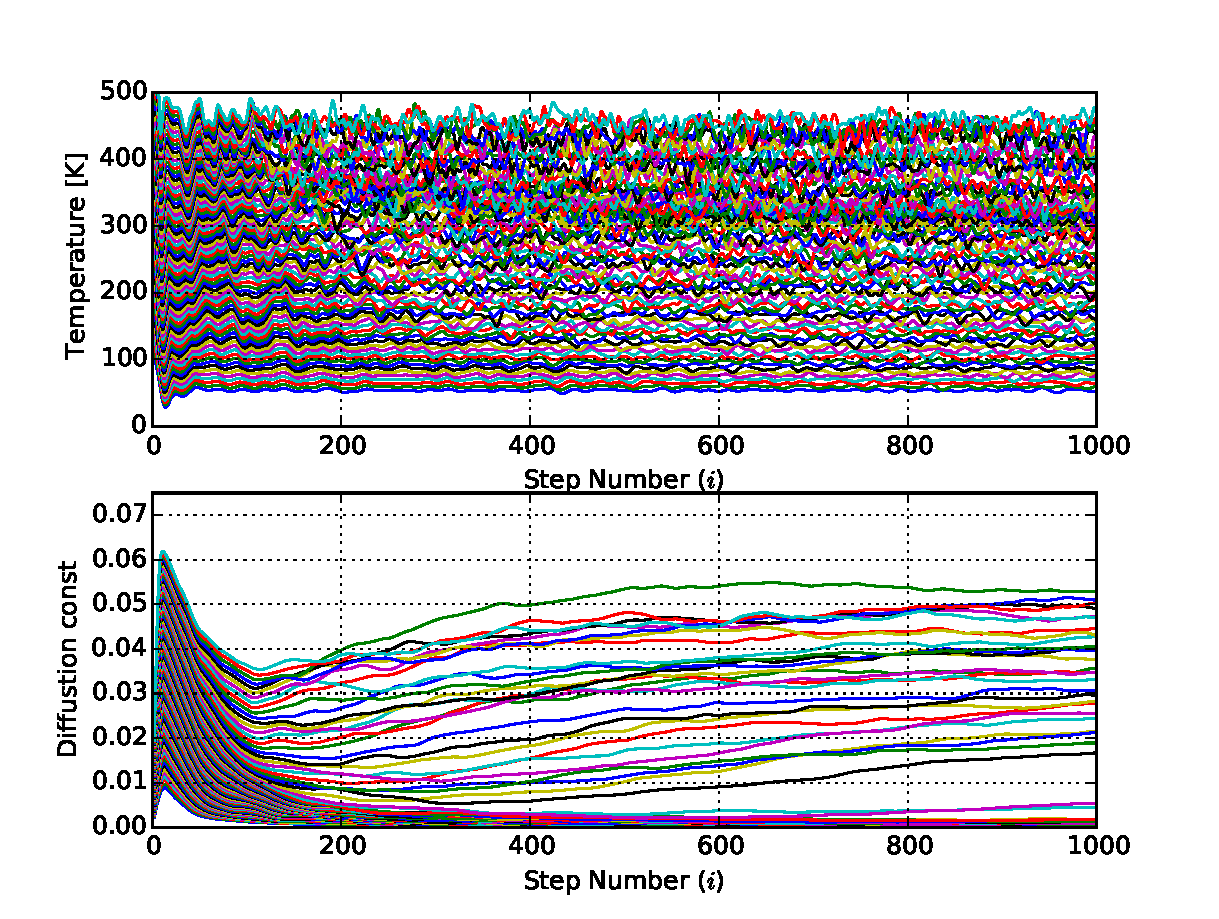
\includegraphics[width=0.5\textwidth]{figures/TDplot.pdf}
	\caption{In the top panel, we show the temperature vs. time
	step number. In the bottom panel, we plot, as a function of
	step number, the diffusion
	constant in units of {\AA}$^2 / s_{\mathrm{MD}}$ where
	$s_{\mathrm{MD}}$ is the unit of time used in the simulations.
	The different lines correspond to simulations with different
	initial temperatures ranging from 100 K to 900 K in steps of
	10 K. Each simulation used 1000 steps and a step size of
	\pwrten{-14} s.}
	\label{fig:TDplot}
\end{figure}

The information in FIG.~\ref{fig:TDplot} can be represented more
succinctly by noting that the temperature ($T$) and $D$ are relatively
constant over the last 200 time steps of all the simulations. Therefore,
we plot $D$ vs. $T$ both averaged over the last 200 time steps in
FIG.~\ref{fig:DavgDplots}. The top panel of FIG.~\ref{fig:DavgDplots}
shows that for all the simulations, $D$ remains roughly constant over
the last 200 time steps. The bottom panel shows a discontinuity in the
diffusion constant as a function of temperature suggesting that the
melting point occurs just above 300 K.

\begin{figure}
\centering
	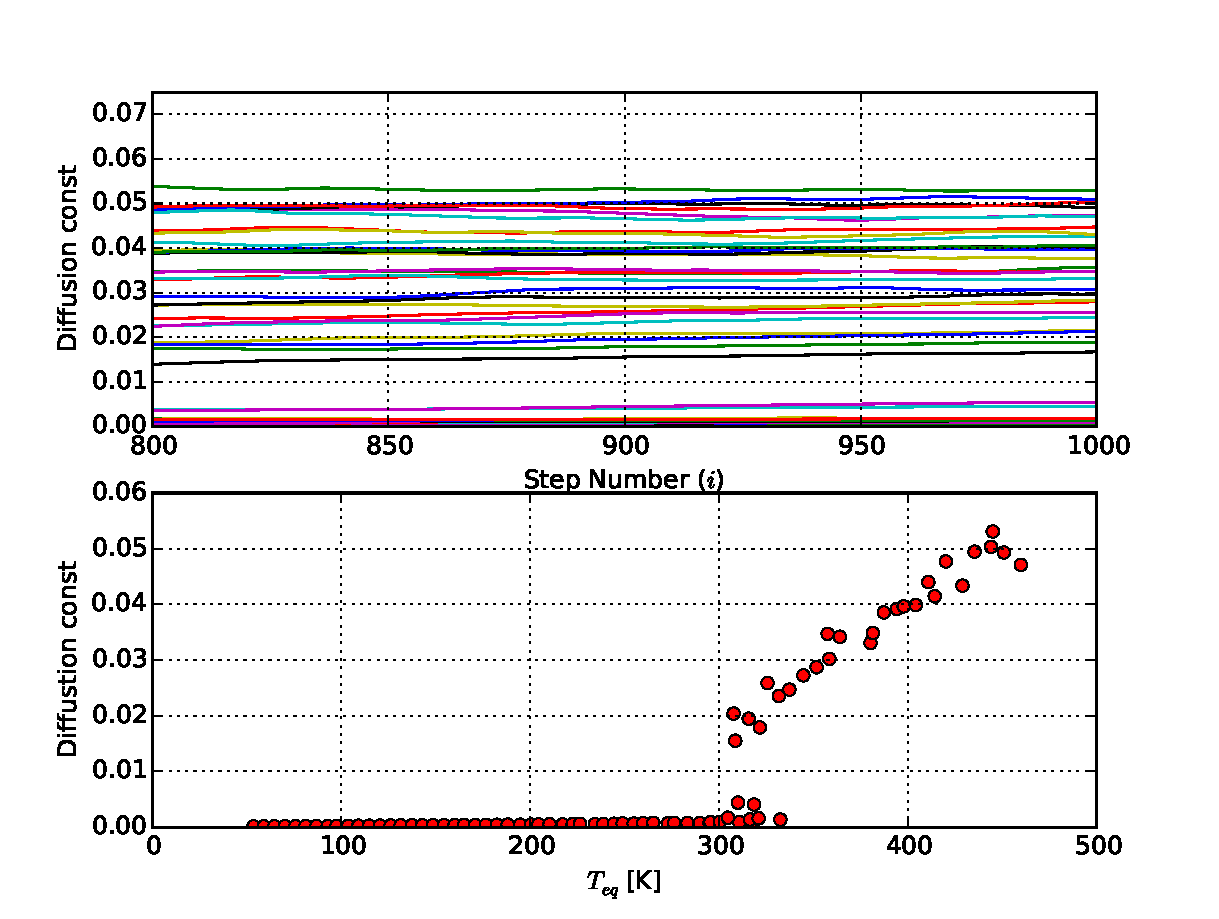
\includegraphics[width=0.5\textwidth]{figures/DavgDplots.pdf}
	\caption{In the top panel, we plot the diffusion constant
	in units of ${\AA} ^2 / s_{\mathrm{MD}}$ vs.
	the time step index. The bottom panel shows the diffusion
	constant vs. the temperature where both observables have
	been averaged over the last 200 time steps.}
	\label{fig:DavgDplots}
\end{figure}

To ensure that the
simulation time wasn't too short to capture the melting process for
systems initialized close to the melting point, we ran two 
batches of simulations with 10000 time steps each. We simulated
systems with $T_eq$ ranging from 280 K to 292.5 K and 195 K to 205 K.
The $D$ vs. time step index from these simulations are shown in
FIG.~\ref{fig:meltPlotsHigh} and FIG.~\ref{fig:meltPlotsLow},
respectively.

\begin{figure}
\centering
	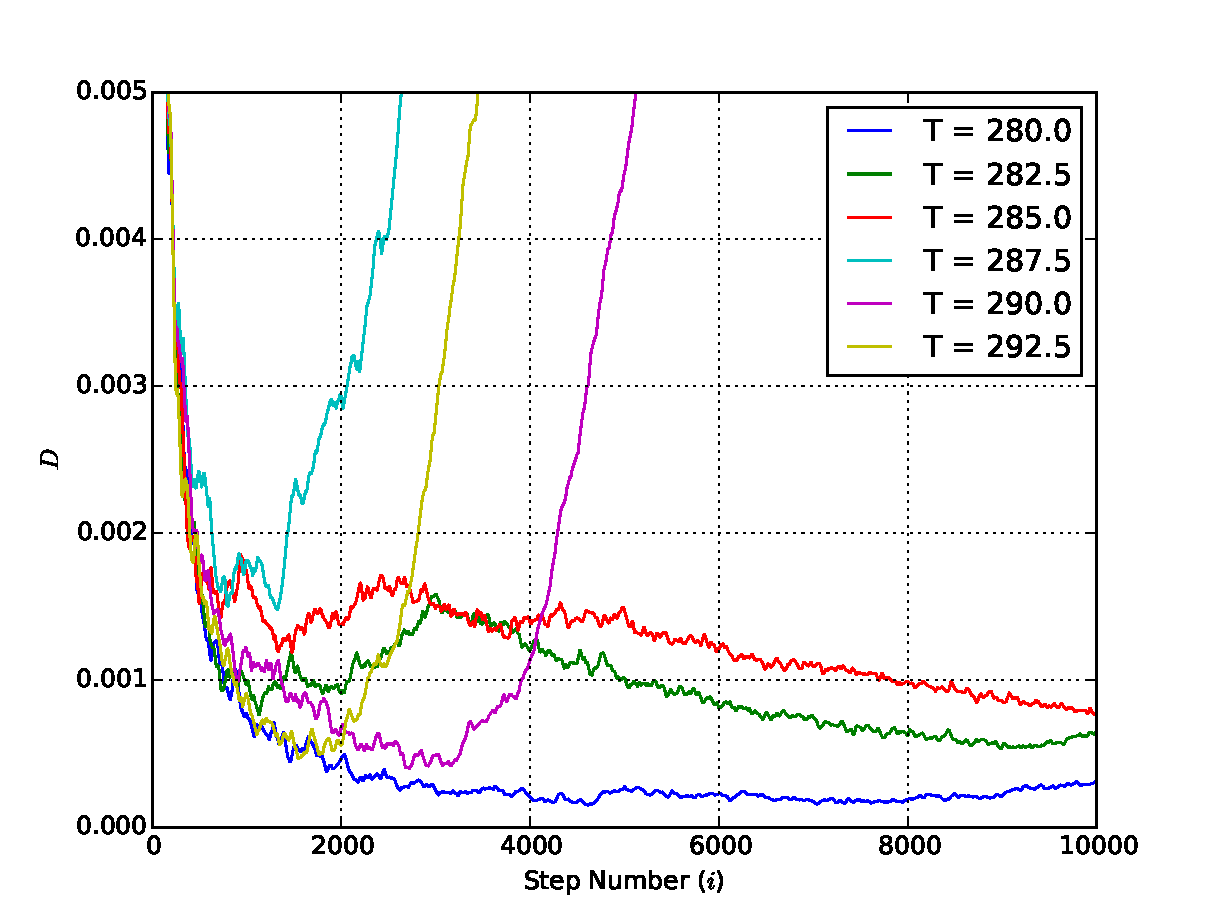
\includegraphics[width=0.5\textwidth]{figures/meltPlots.pdf}
	\caption{Diffusion constant vs. time step for systems with 5
	different $T_ep$ raging from 280 K to 292.5 K in steps of 2.5 K. Each
	simulation was run with 10000 time steps.}
	\label{fig:meltPlotsHigh}
\end{figure}

\begin{figure}
\centering
	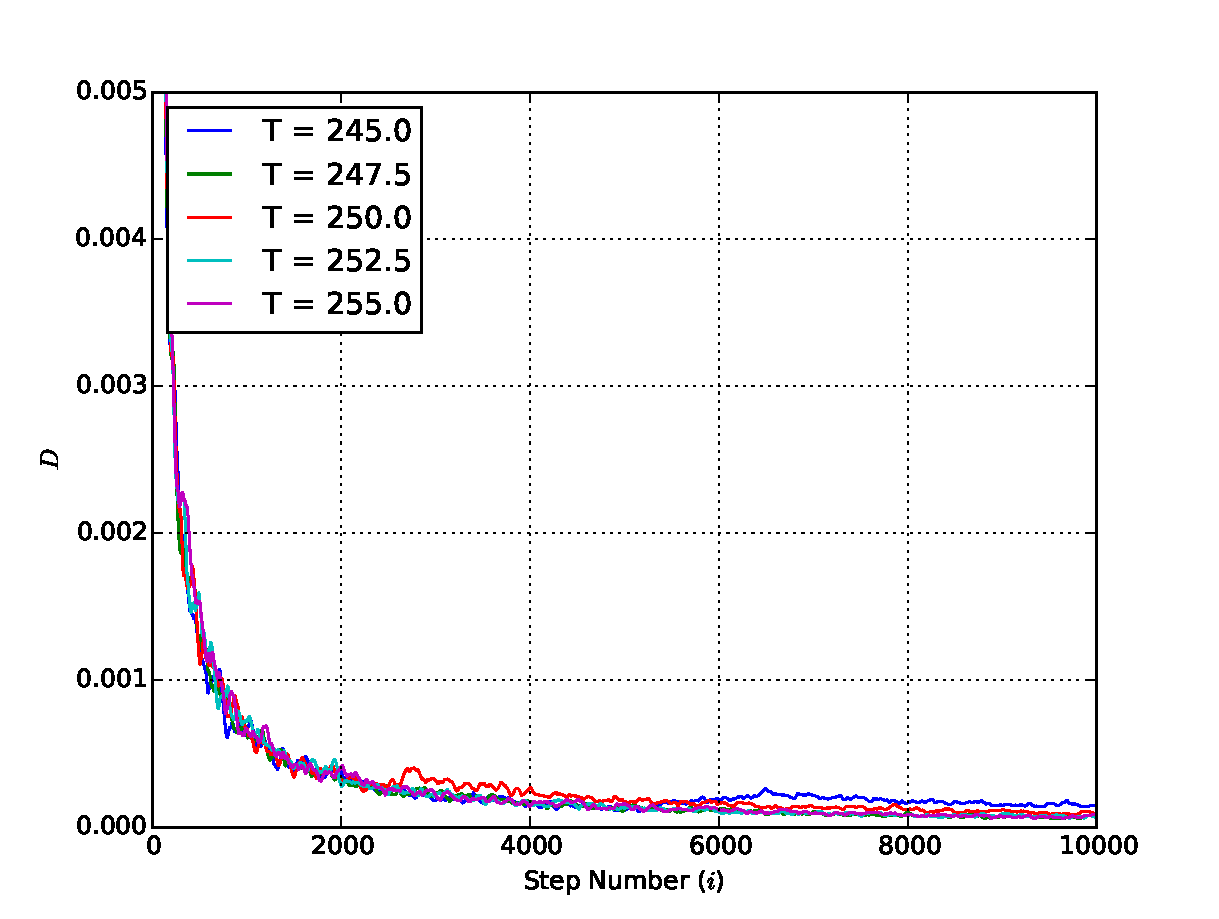
\includegraphics[width=0.5\textwidth]{figures/meltPlotsLow.pdf}
	\caption{Diffusion constant vs. time step for systems with 5
	different $T_ep$ raging from 245 K to 255 K in steps of 2.5 K. Each
	simulation was run with 10000 time steps.}
	\label{fig:meltPlotsLow}
\end{figure}






%\begin{figure}
%\centering
%	\includegraphics[width=0.5\textwidth]{figures/dnit2.pdf}
%	\caption{The number of similarity transformations needed to
%	diagonalize the matrix is plotted against the matrix
%	dimensionality. A quadratic fit gives a $2 N^2 - 8 N$ dependence
%	of the number of similarity transformations on the dimensionality
%	$N$.}
%	\label{fig:dnit}
%\end{figure}


%\begin{figure}
%\centering
%	\includegraphics[width=0.5\textwidth]{figures/gsw.pdf}
%	\caption{Ground state wavefunctions for different oscillator
%	strengths and no interaction between the electrons.
%	The weakest potential ($\omega = 0.01$) is shown in black and the
%	strongest potential ($\omega = 5$) is plotted in green.
%	The wavefunctions have been scaled to the $\omega = 5$ wavefunction.}
%	\label{fig:gsw}
%\end{figure}

%\begin{figure}[hbtp]
%\includegraphics[scale=0.4]{test1.pdf}
%\caption{Exact and numerial solutions for $n=10$ mesh points.} 
%\label{fig:n10points}
%\end{figure}



%\begin{figure}[h!]
%\centering
%	\includegraphics[width=0.5\textwidth]{figures/CIwvfn.pdf}
%	\caption{Ground state wavefunctions vs. separation distance for two
%	Coulomb-interacting electrons in a harmonic oscillator potential.}
%	\label{fig:ci}
%\end{figure}

\section{Conclusions}

Future work: pressure, other observables ...

%\begin{thebibliography}{99}
%%\bibitem{miller2006} G.~A.~Miller, A.~K.~Opper, and E.~J.~Stephenson, Annu.~Rev.~Nucl.~Sci.~{\bf 56}, 253 (2006).
%\end{thebibliography}


\bibliographystyle{plainnat}
\bibliography{refs}

\end{document}